\documentclass{standalone}
\usepackage{tikz}
\usepackage{pgfplots}
\pgfplotsset{compat=newest}
\usepackage{amsmath}
\usepackage[american]{circuitikz}
\usepackage{cmbright}

\definecolor{myred}{RGB}{170,0,0}
\definecolor{myblue}{RGB}{0,0,220}
\definecolor{mygreen}{RGB}{0,150,0}
\definecolor{myorange}{RGB}{255,127,0}
\definecolor{mybrown}{RGB}{150,75,0}

\begin{document}
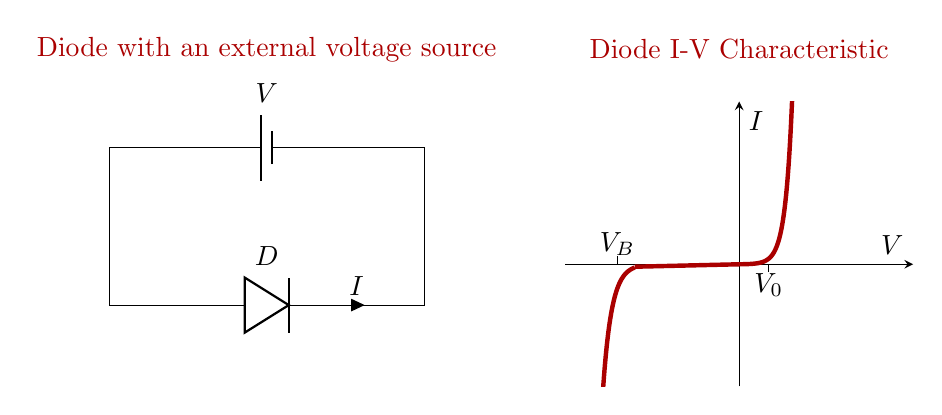
\begin{tikzpicture}
    % Diode circuit
    \begin{scope}
        \node[anchor=center, color=myred] at (2, 3.25) {Diode with an external voltage source};
        \draw (0,0) to[D, l=$D$, , i^>=$I$] ++(4, 0) 
              to ++(0, 2) 
              to[battery1, l_=$V$, invert] ++(-4, 0) 
              to ++(0, -2);
    \end{scope}

    % Diode I-V characteristic
    \begin{scope}[yshift=0cm, xshift=8cm]
        \node[anchor=center, color=myred] at (0, 3.25) {Diode I-V Characteristic};
        \begin{axis}[
            at={(0,0.5)},
            anchor=origin,
            width=6cm,
            height=5.2cm,
            xmin=-5, xmax=5,
            ymin=-1500, ymax=2000,
            domain=-2:0.7,
            samples=200,
            axis lines=center,
            xlabel={$V$},
            ylabel={$I$},
            xtick=\empty,
            ytick=\empty,
            clip=true,
        ]
        % Parametric forward bias: V = x, I = f(V)
        \addplot[myred, ultra thick, domain=0:2] (x, {(exp(5 * x)-1)});

        % Parametric reverse bias
        \addplot[myred, ultra thick, domain=-3:0] (x, {10 * x});
        \addplot[myred, ultra thick, domain=-5:-3] (x, {-40 * (exp(4.0 * (-x - 3)))});
        
        % Mark the V0 voltage.
        \draw[black, thin] (0.85, 0) -- (0.85, -100);
        \node [anchor=center, color=black] at (0.85, -250) {$V_0$};

        % Mark the breakdown voltage.
        \draw[black, thin] (-3.5, 0) -- (-3.5, 100);
        \node [anchor=center, color=black] at (-3.5, 250) {$V_B$};
        \end{axis}
    \end{scope}

\end{tikzpicture}
\end{document}